\begin{frame}{Project Requirements}


    \begin{columns}
        \begin{column}{0.4\textwidth}
        \begin{itemize}
            \item ROS 2 framework
            \item Flight stability
            \item Real-time image processing
            \item SLAM
            \item Obstacle avoidance
            \item Autonomous navigation and landing
        \end{itemize}
        \end{column}
        \begin{column}{0.6\textwidth}  %%<--- here
            \begin{figure}
                \centering
                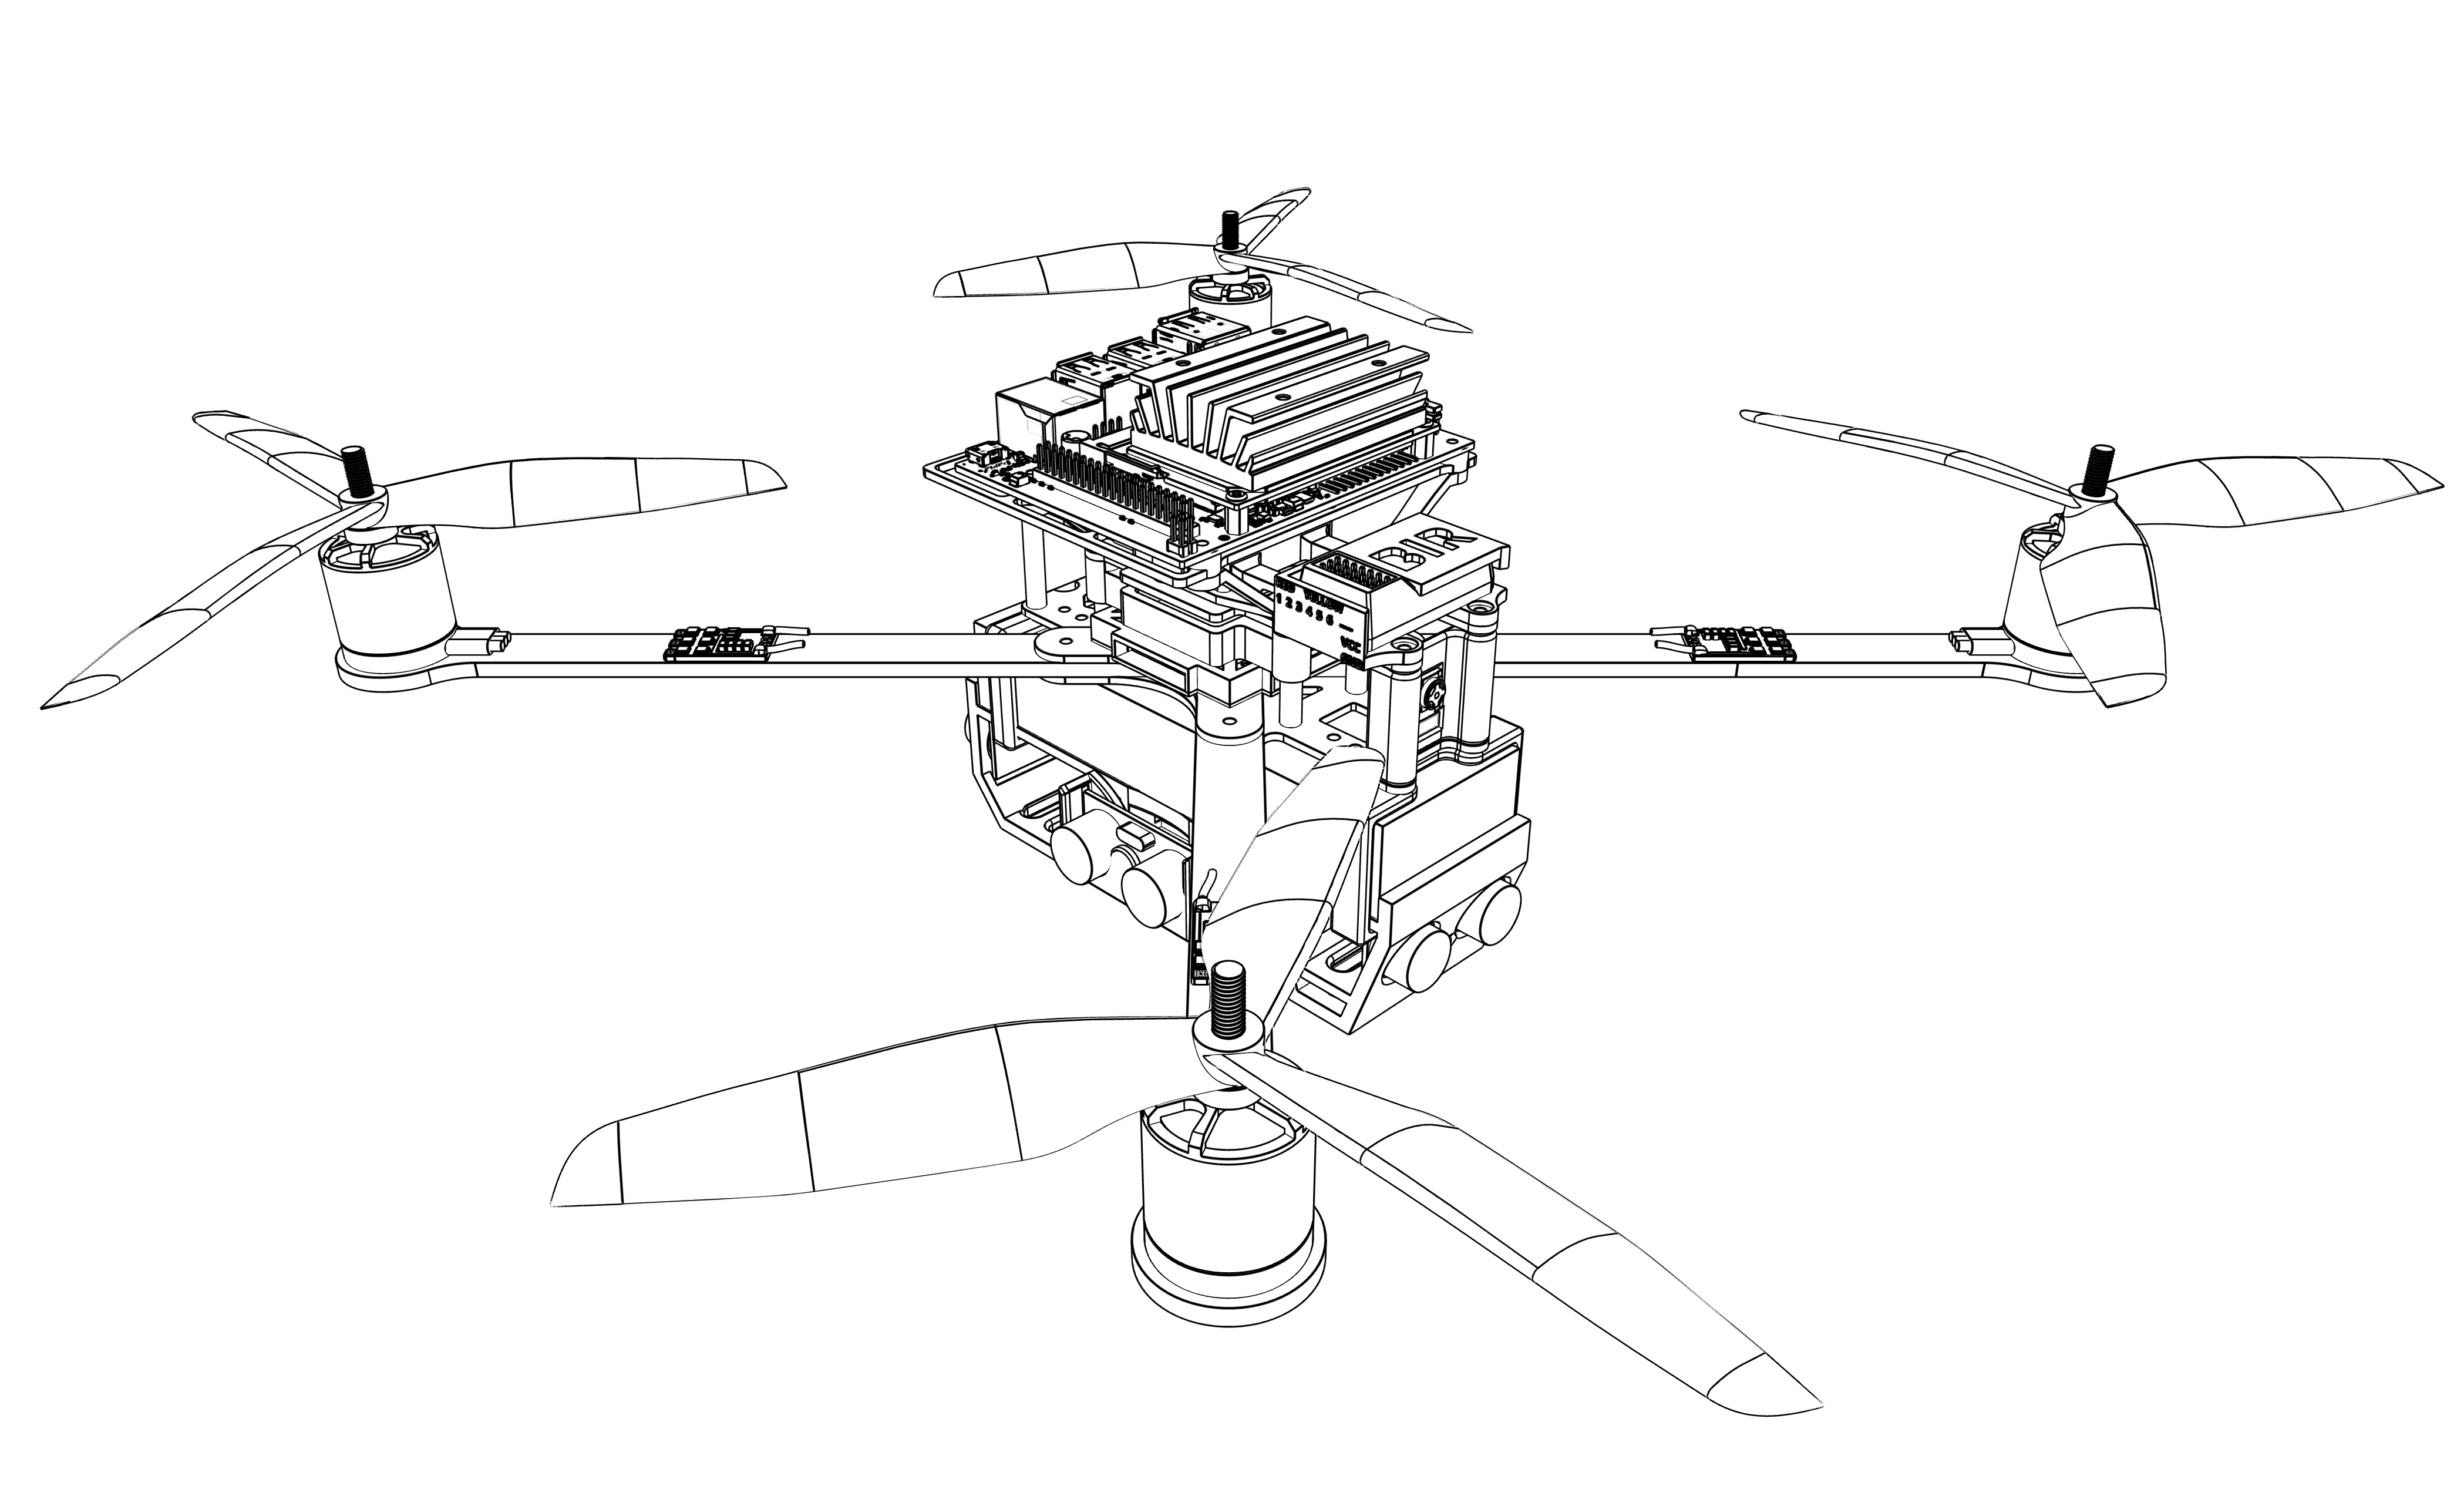
\includegraphics[width=1\textwidth]{img/carcara2.png}
                \label{fig:carcara2}
            \end{figure}
        \end{column}
    \end{columns}
\end{frame}

\begin{frame}{Objective}


    \begin{columns}
        \begin{column}{0.4\textwidth}
        \begin{itemize}
            \item Build a research drone with the potential to autonomously explore unknown environments, avoid obstacles and detect areas of interest.
            % \item Autonomous landing on a fiducial mark
        \end{itemize}
        \end{column}
        \begin{column}{0.6\textwidth}  %%<--- here
            \begin{figure}
                \centering
                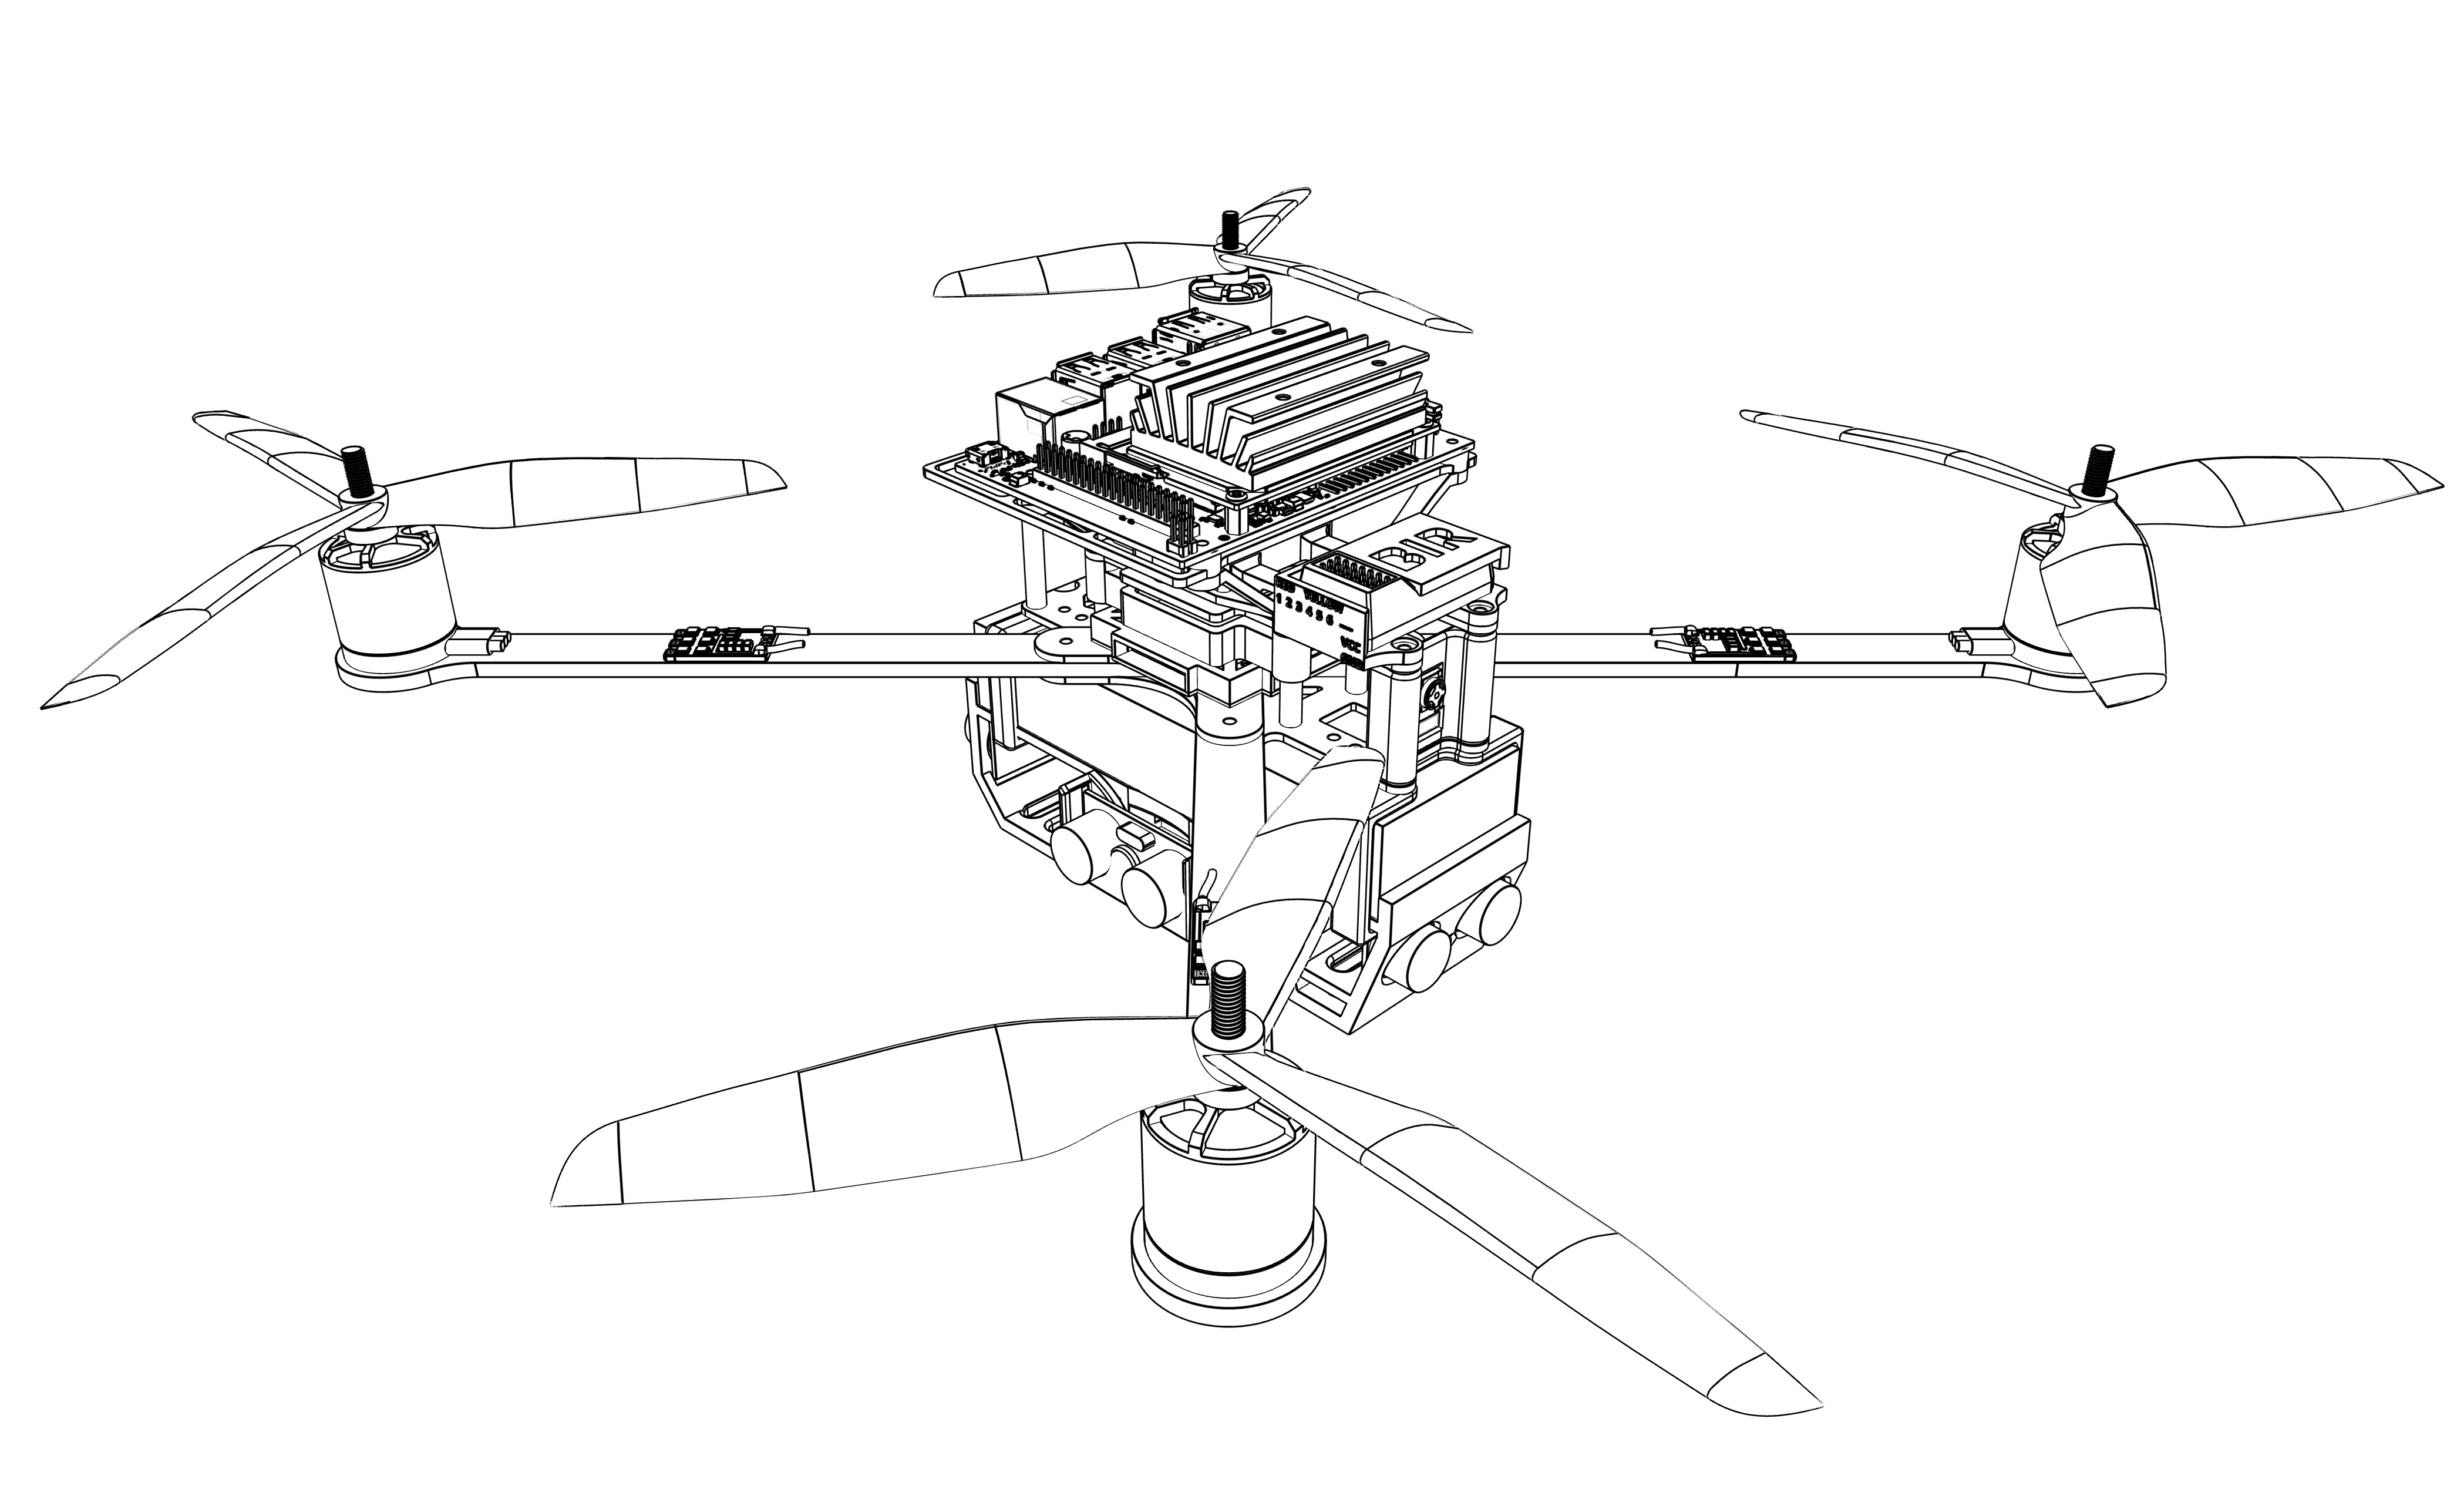
\includegraphics[width=1\textwidth]{img/carcara2.png}
                \label{fig:carcara3}
            \end{figure}
        \end{column}
    \end{columns}
\end{frame}

% \begin{frame}{About the System}


% \begin{columns}
%         \begin{column}{0.4\textwidth}
%         \begin{itemize}
%             \item Underactuated system
%             \item 4 actuators, 6 degrees of freedom
%             % \item Autonomous landing on a fiducial mark
%         \end{itemize}
%         \end{column}
%         \begin{column}{0.6\textwidth}  %%<--- here
%             \begin{figure}
%                 \centering
%                 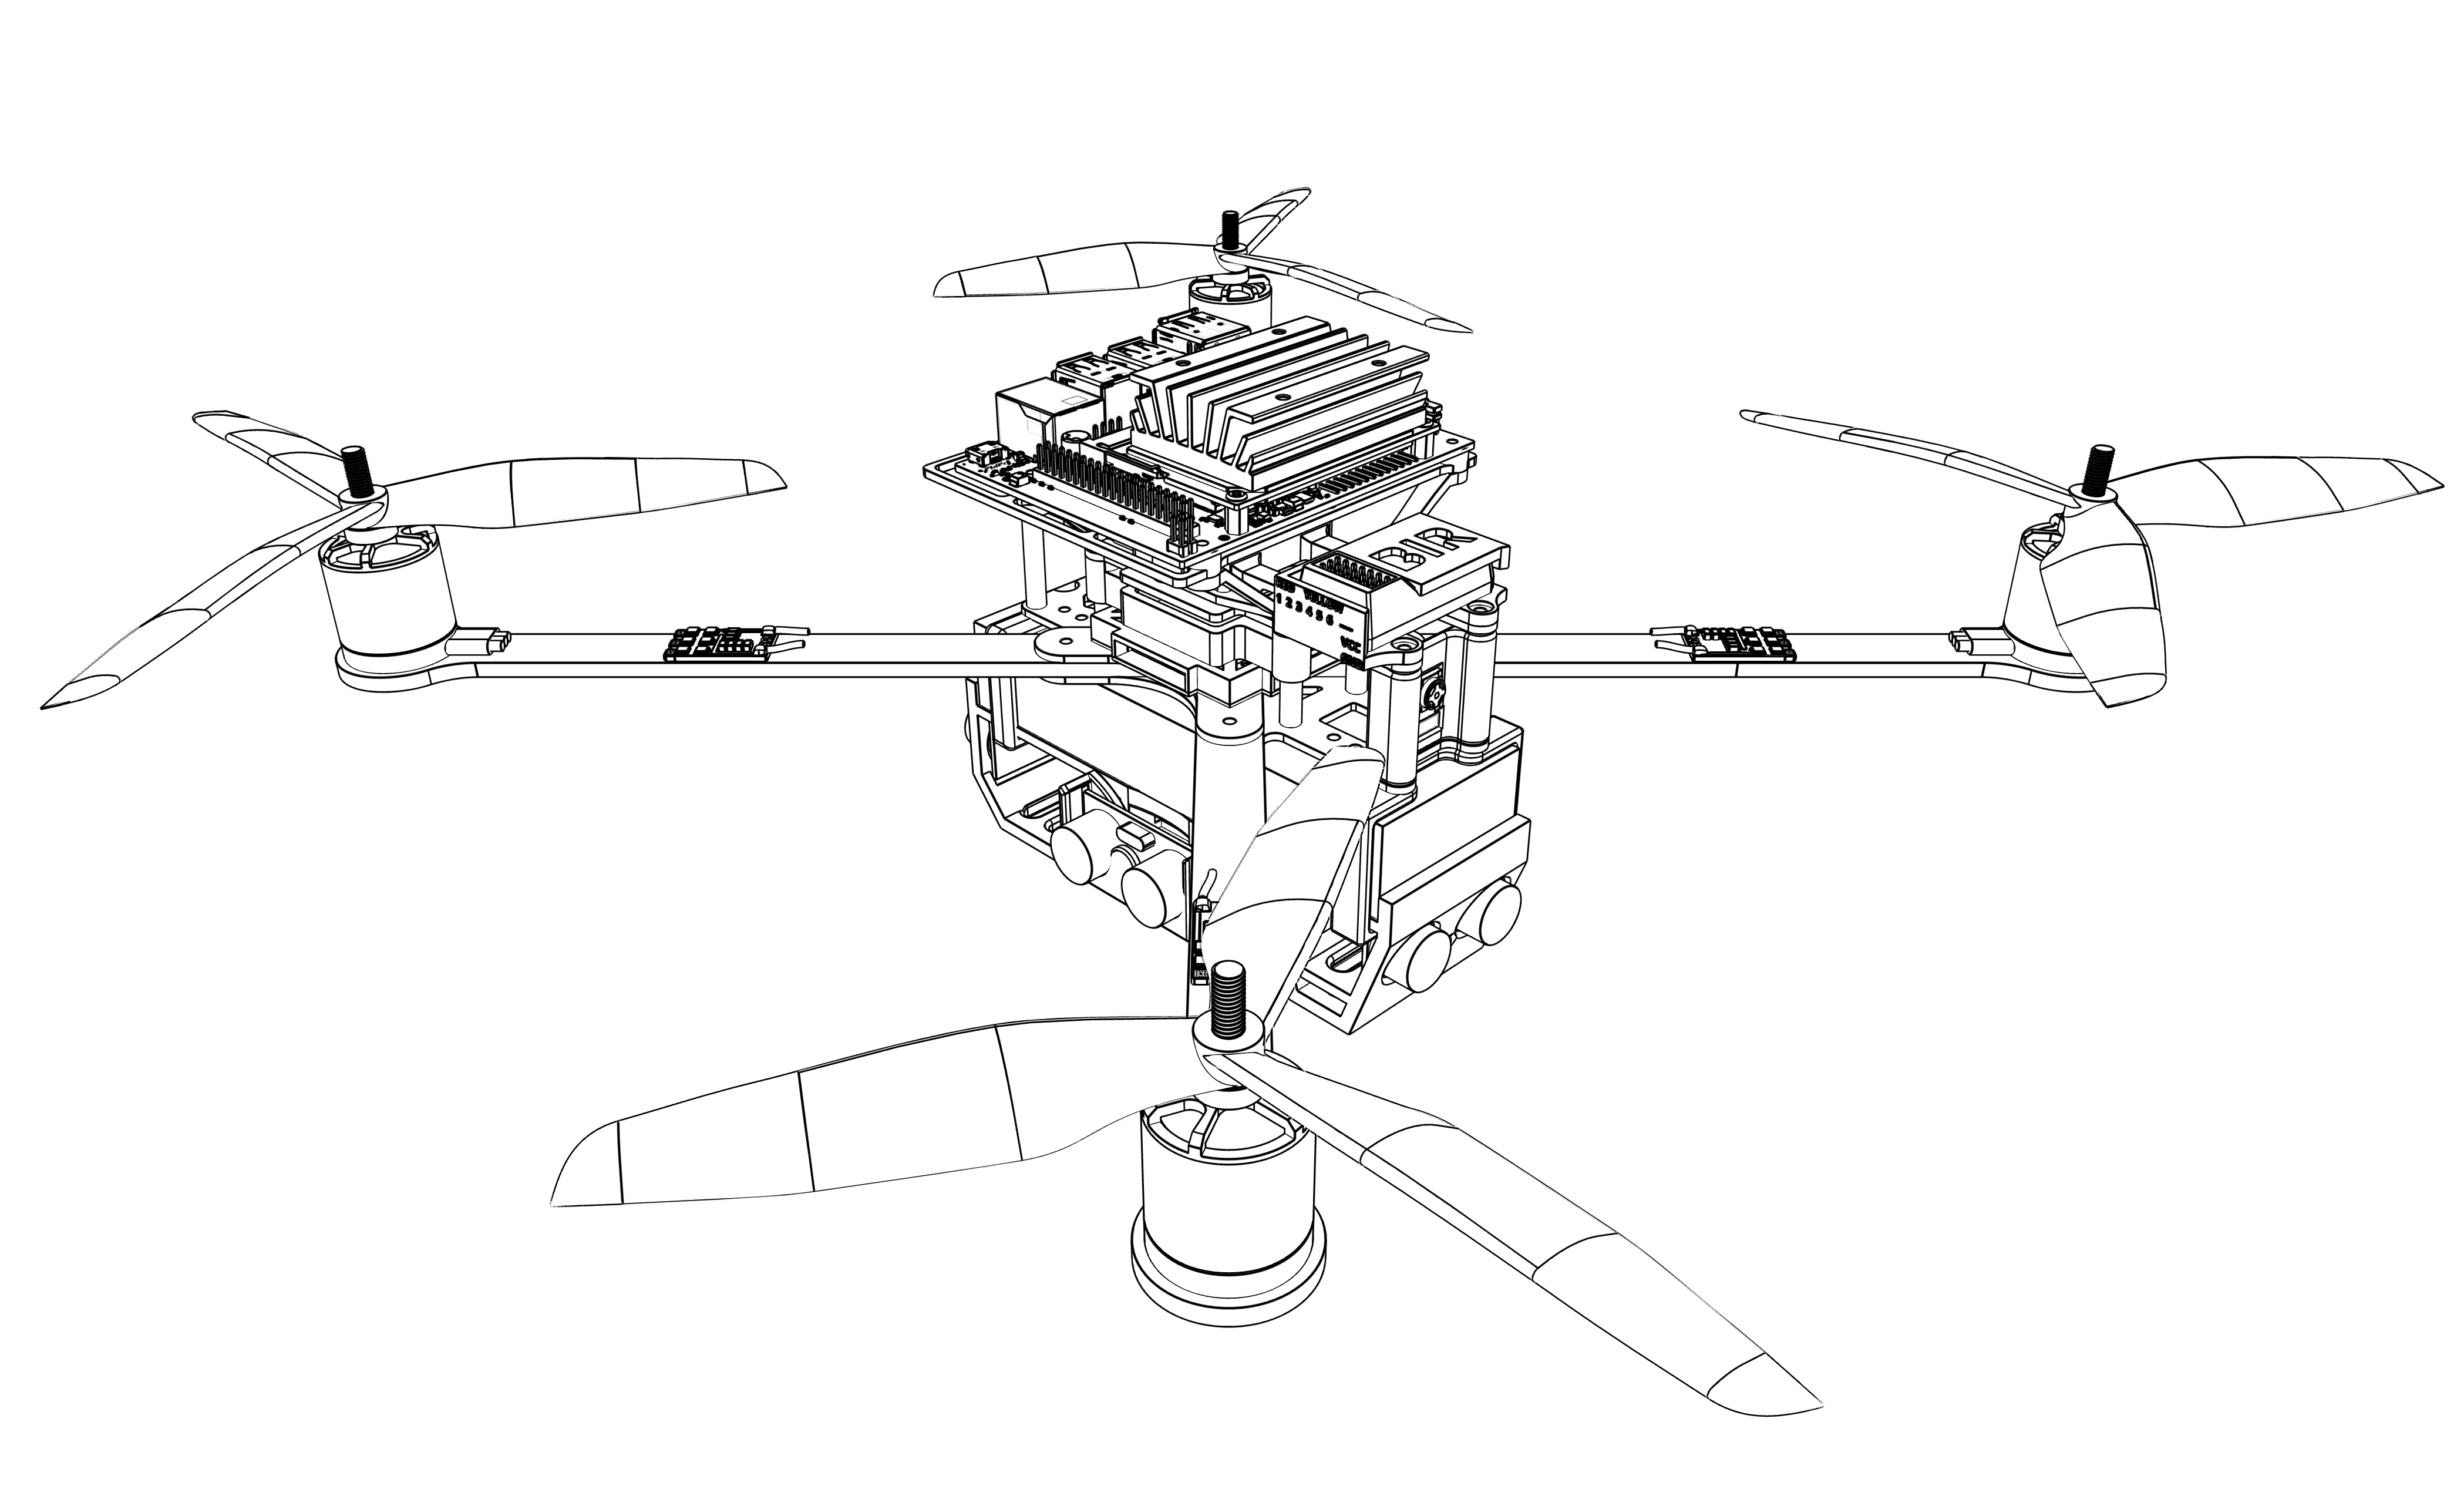
\includegraphics[width=1\textwidth]{img/carcara2.png}
%                 \label{fig:carcara2}
%             \end{figure}
%         \end{column}
%     \end{columns}
% \end{frame}

% \begin{frame}{About the System}


% \begin{columns}
%         \begin{column}{0.4\textwidth}
%         \begin{itemize}
%             \item Underactuated system
%             \item 4 actuators, 6 degrees of freedom
%             % \item Autonomous landing on a fiducial mark
%         \end{itemize}
%         Assumptions:
%         \begin{itemize}
%             \item The quadcopter is a rigid body.
%             \item The structure is symmetric.
%             \item The center of mass of the system coincides with the origin of the coordinate system.
%         \end{itemize}
%         \end{column}
%         \begin{column}{0.6\textwidth}  %%<--- here
%             \begin{figure}
%                 \centering
%                 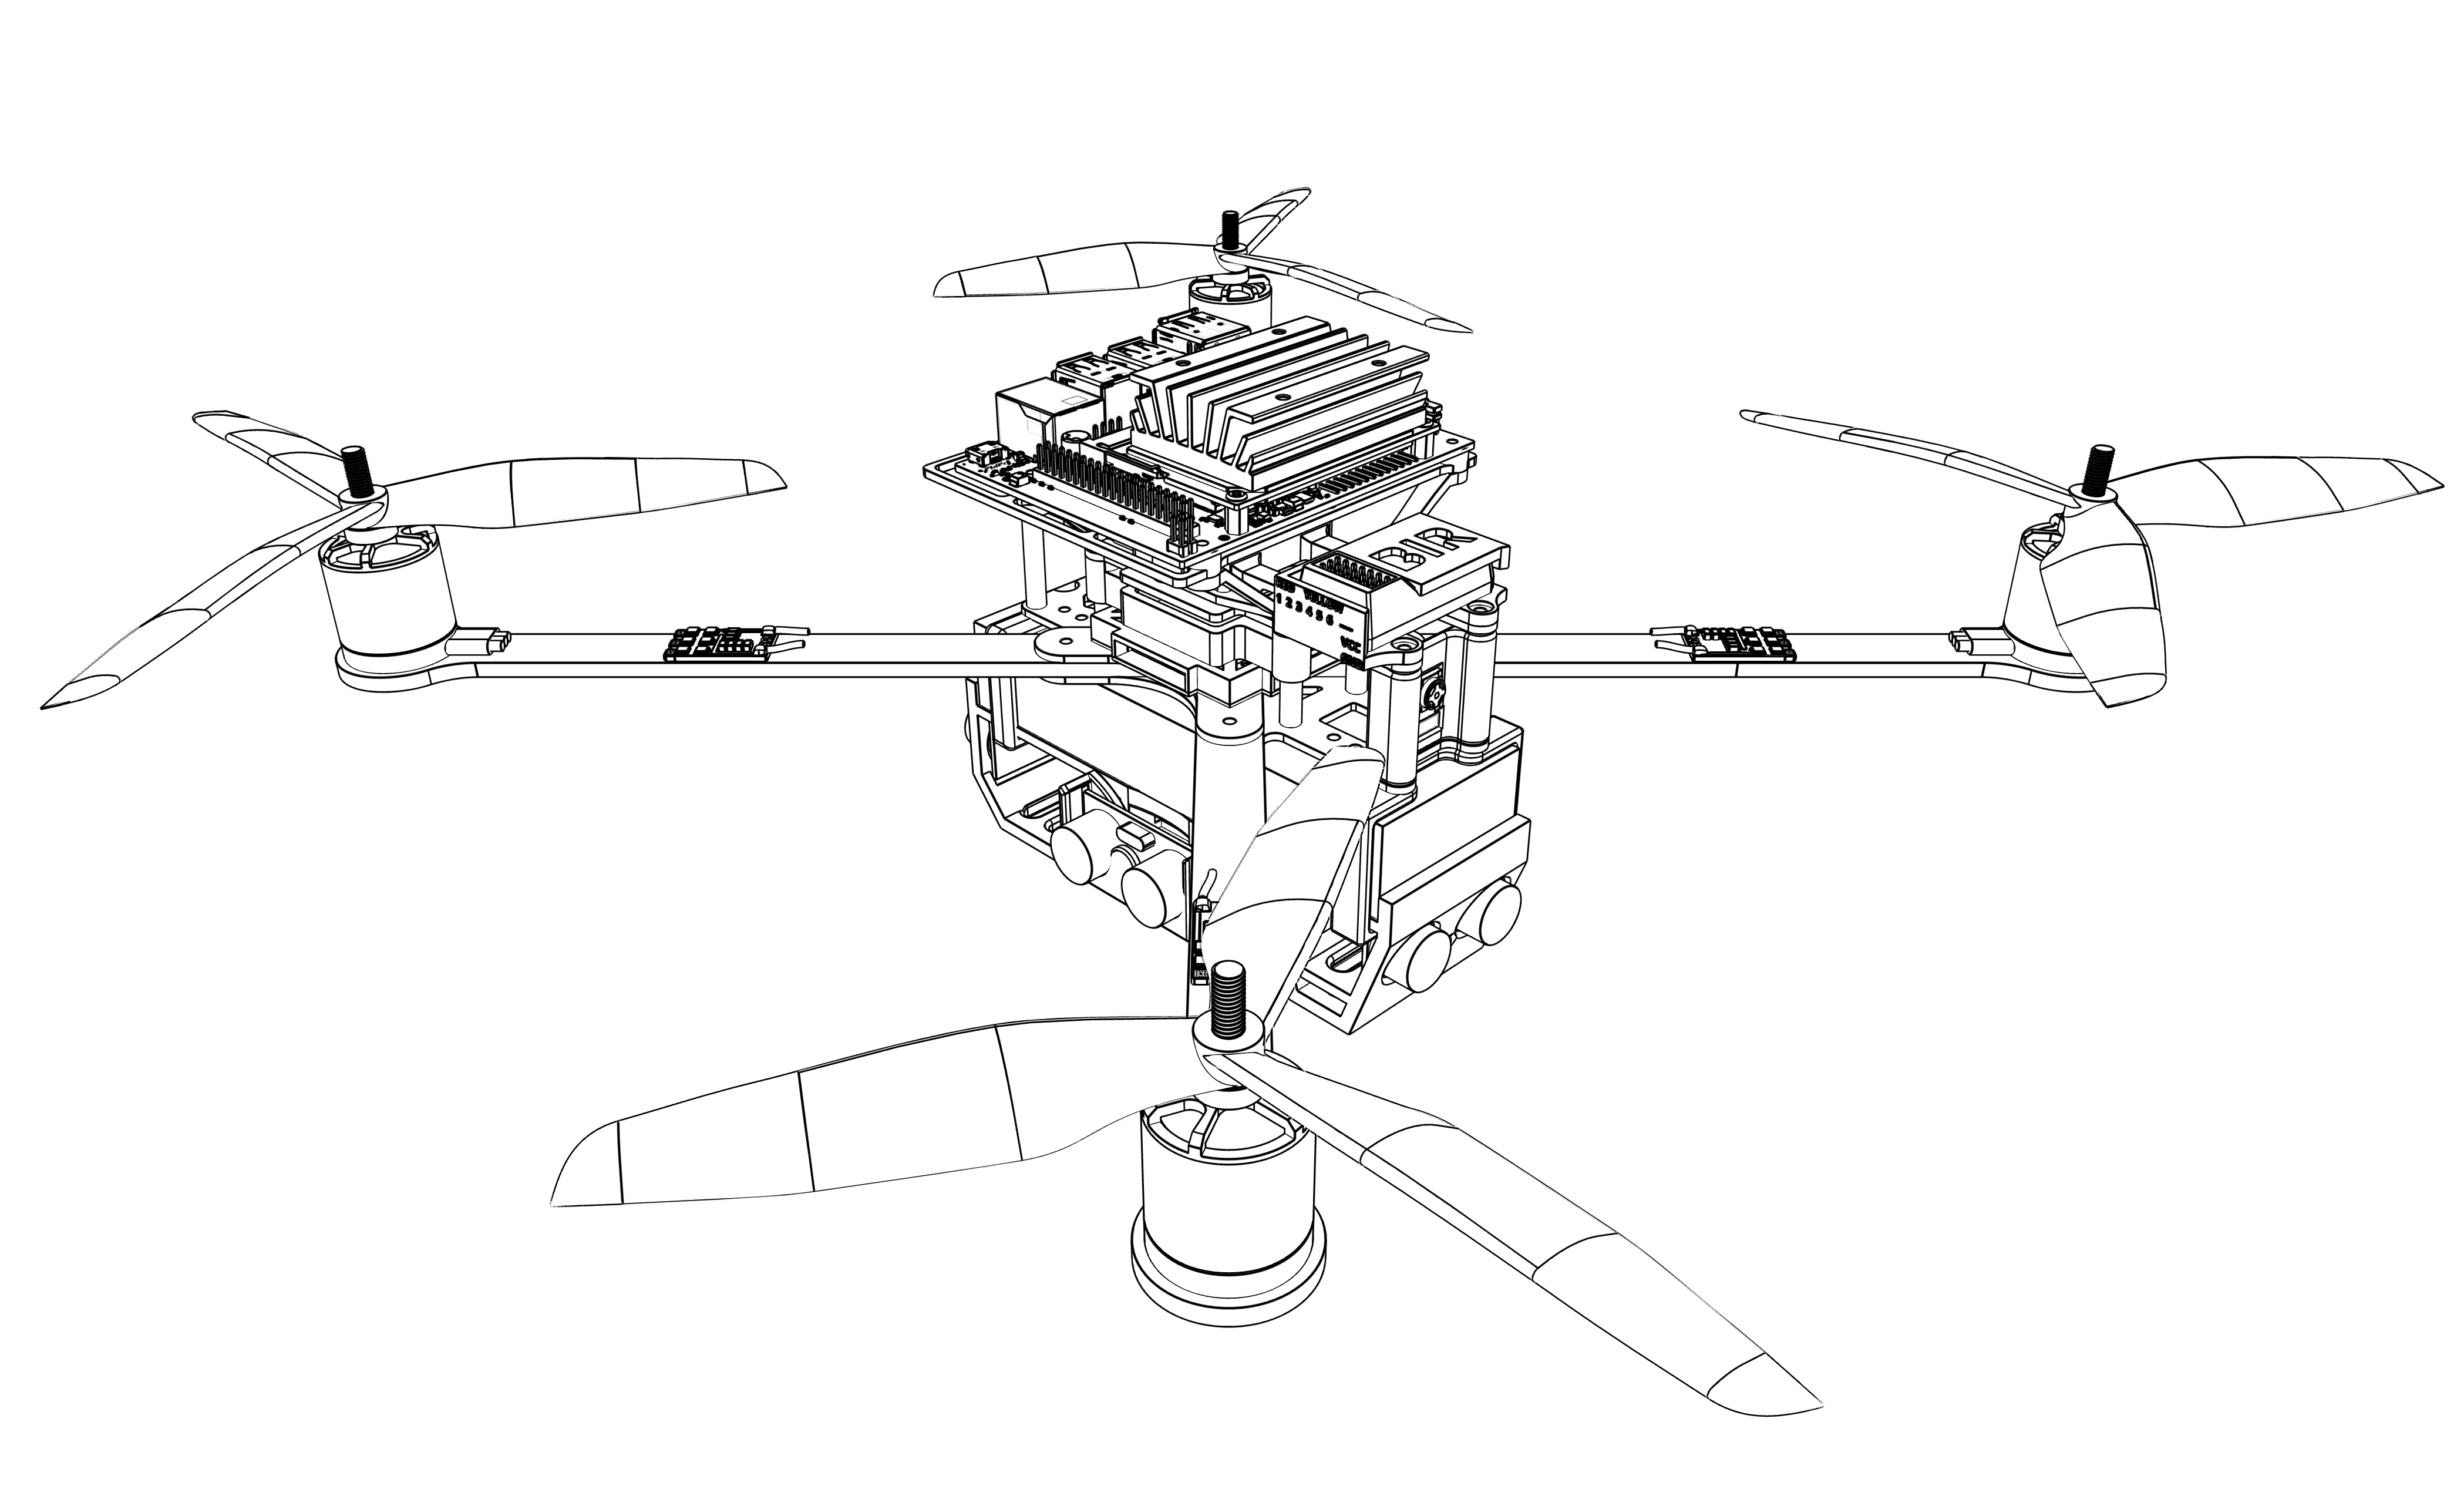
\includegraphics[width=1\textwidth]{img/carcara2.png}
%                 \label{fig:carcara2}
%             \end{figure}
%         \end{column}
%     \end{columns}
% \end{frame}

% \begin{frame}{Mathematical Model}
%     \begin{itemize}
%         % \item Formulação de Newton-Euler
%         \item Rotational dynamics
%         \item 3 Degrees of freedom
%     \end{itemize}


% \begin{columns}
% \begin{column}{0.4\textwidth}
% \begin{align*}\resizebox{.6\hsize}{!}{
%         \begin{dcases}
%             &\dot{\theta} = p+ r\,cos(\phi )\,{tan}(\theta)+q\,sen(\varphi )\,{tan}({\theta})\\
%             &\dot{\phi} = q\,cos(\phi )-r\,sen(\phi )\\
%             &\dot{\psi} = \frac{r\,cos(\phi )}{cos({\theta})}+\frac{q\,sen(\phi )}{cos({\theta})}\\
%             &\dot{p} = \frac{I_{y} - I_{z}}{I_{x}}q r + \frac{\tau_{x}}{I_{x}}\\
%             &\dot{q} = \frac{I_{z} - I_{x}}{I_{y}}p r + \frac{\tau_{y}}{I_{y}}\\
%             &\dot{r} = \frac{I_{x} - I_{y}}{I_{z}}p q + \frac{\tau_{z}}{I_{z}}\\
%             &\tau_{x} = b l\, sen(\pi/4) (\Omega_{1}^{2} + \Omega_{2}^{2} - \Omega_{3}^{2} - \Omega_{4}^{2})\\
%             &\tau_{y} = b l\, sen(\pi/4) (\Omega_{1}^{2} + \Omega_{4}^{2} - \Omega_{2}^{2} - \Omega_{3}^{2})\\
%             &\tau_{z} = d (\Omega_{2}^{2} + \Omega_{4}^{2} - \Omega_{1}^{2} - \Omega_{3}^{2})
%         \end{dcases}}
%     \end{align*}
% \end{column}
% \begin{column}{0.6\textwidth}  %%<--- here
%     % \begin{center}[width=1.1\textwidth]
%      \begin{figure}
%          \centering
%          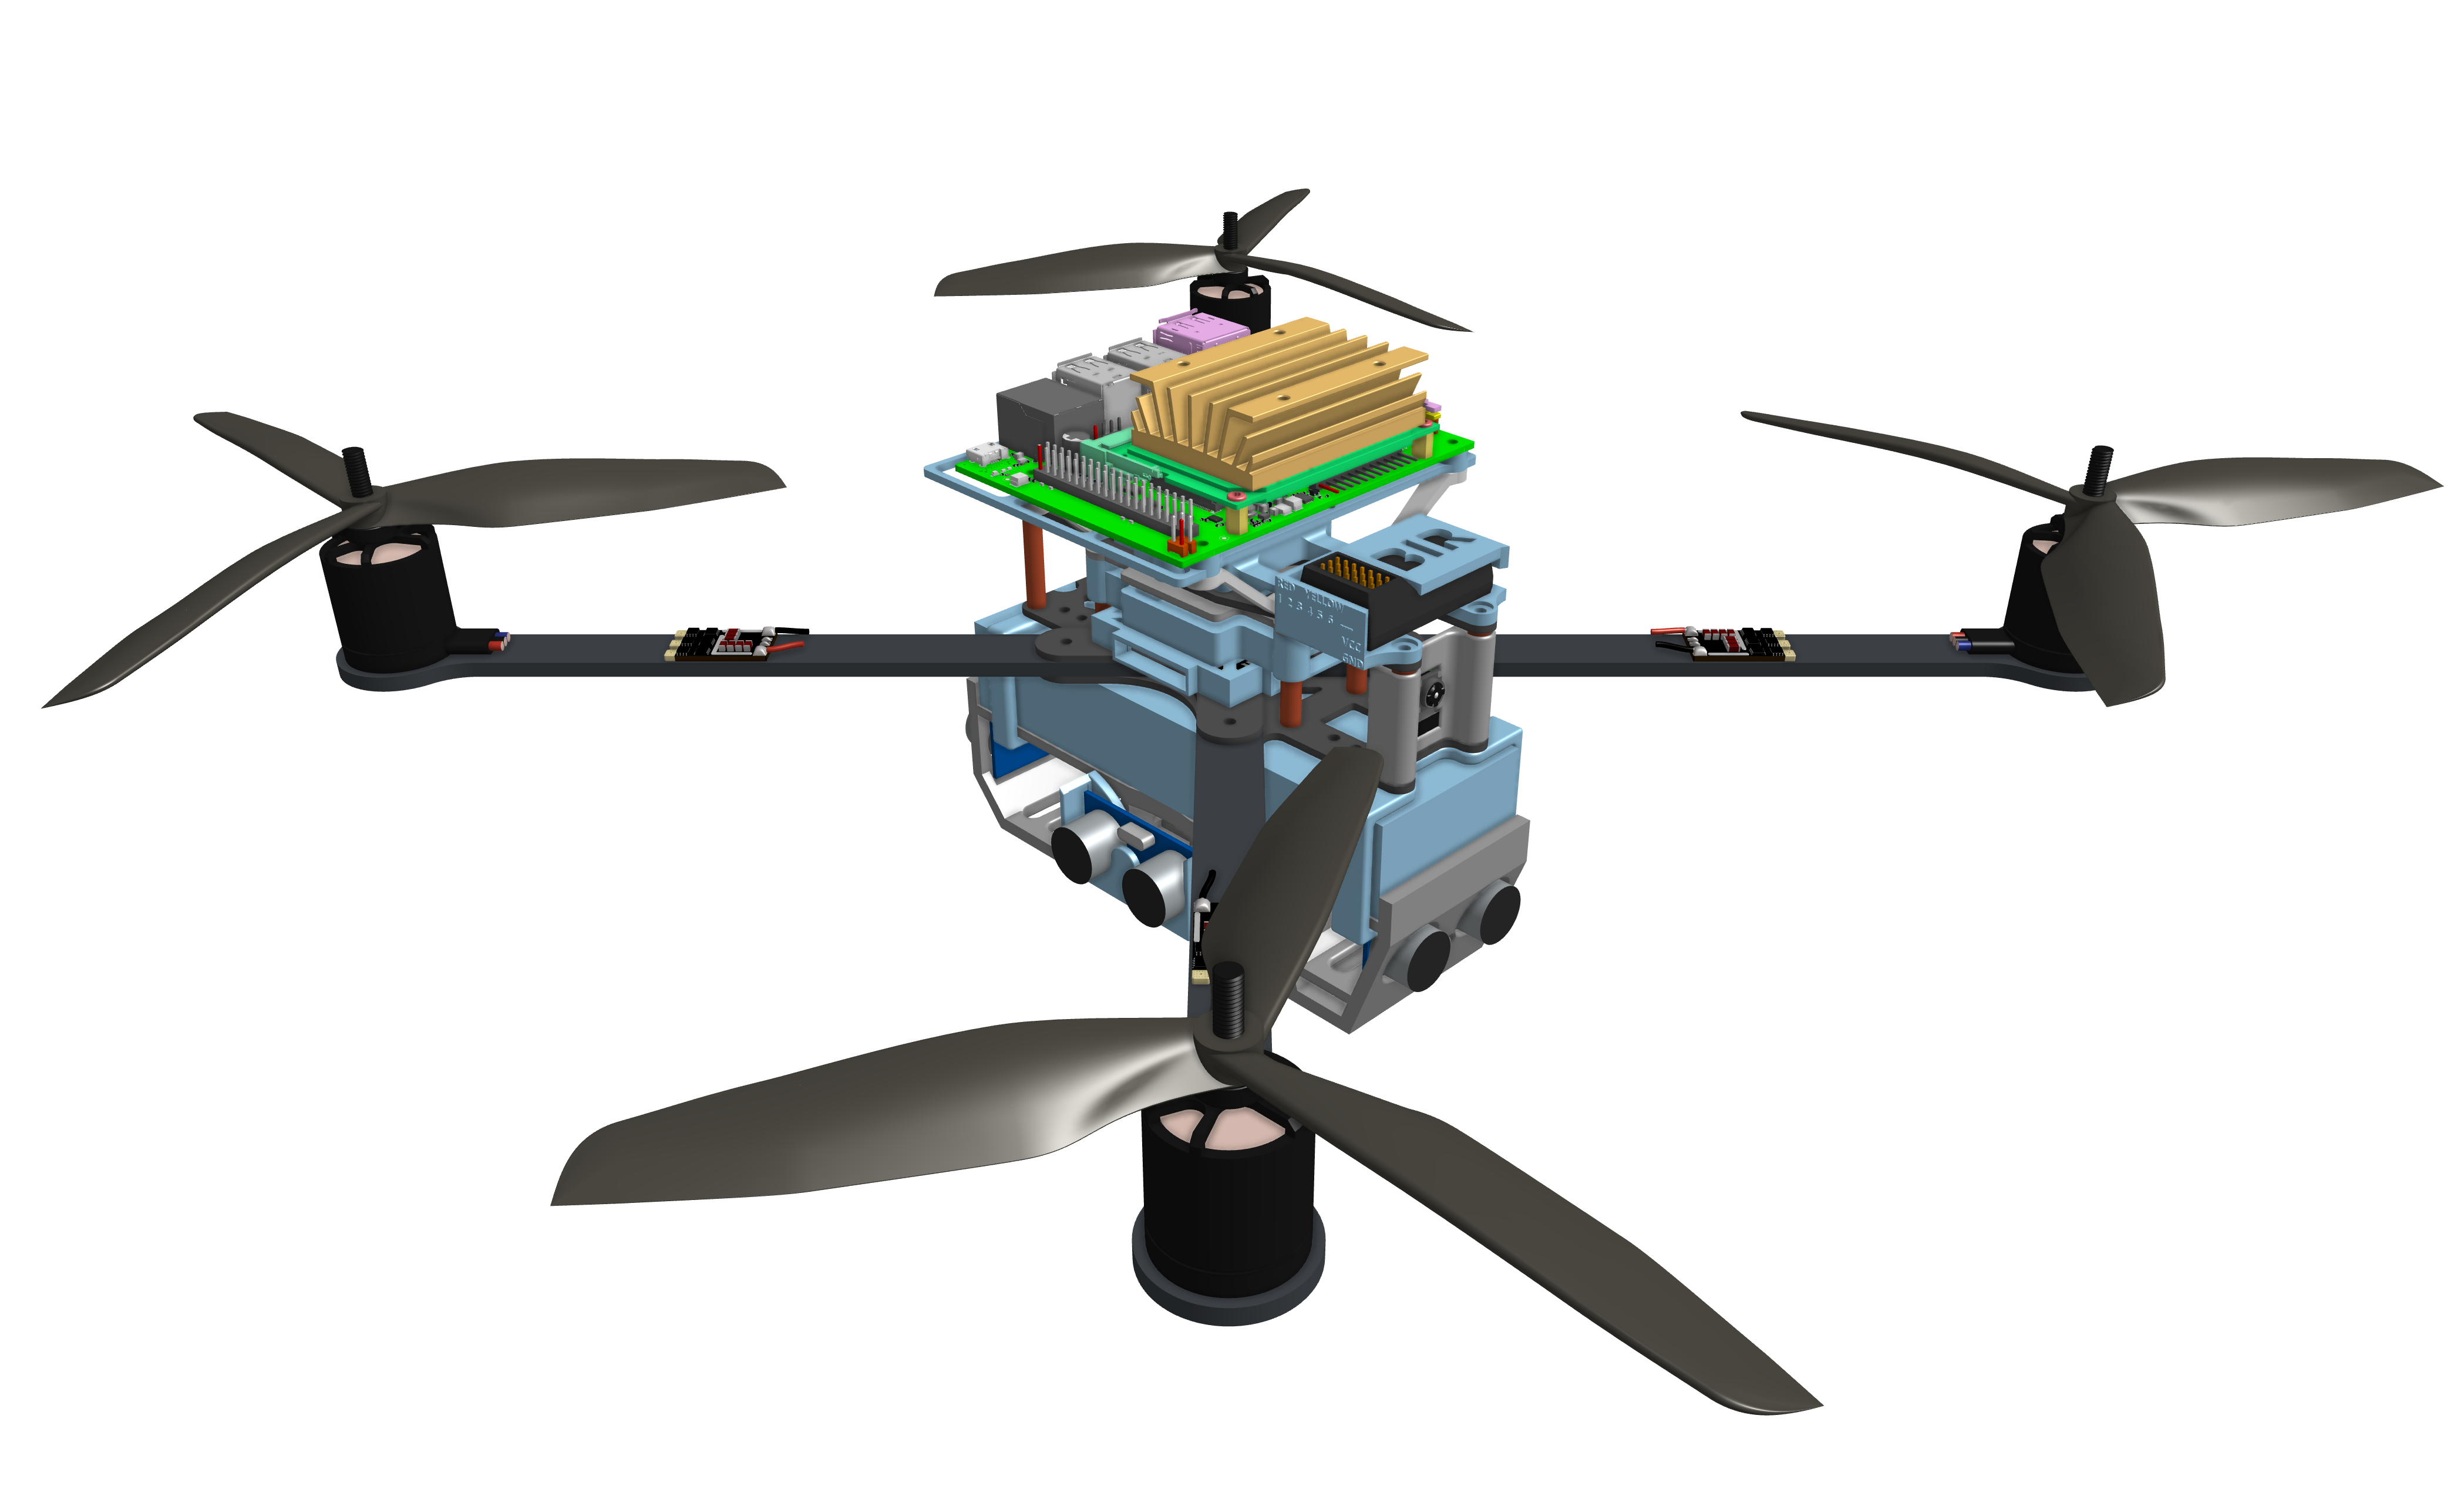
\includegraphics[width=1\textwidth]{img/carcara3.png}
%      \end{figure}
%     %  \end{center}
% \end{column}
% \end{columns}

% \end{frame}



% \begin{frame}{Mathematical Model}
%     % Sendo $\tau_{x},\tau_{y}$ e $\tau_{z}$ dados por
%     % \begin{align*}
%     % \begin{dcases}
%     %     &\tau_{x} = b l s(\pi/4) (\Omega_{1}^{2} + \Omega_{2}^{2} - \Omega_{3}^{2} - \Omega_{4}^{2})\\
%     %     &\tau_{y} = b l s(\pi/4) (\Omega_{1}^{2} + \Omega_{4}^{2} - \Omega_{2}^{2} - \Omega_{3}^{2})\\
%     %     &\tau_{z} = d (\Omega_{2}^{2} + \Omega_{4}^{2} - \Omega_{1}^{2} - \Omega_{3}^{2})
%     % \end{dcases}
%     % \end{align*}
%             \begin{itemize}
%                 \item The actuators have the same dynamics.
%                 \item The thrust factor ($b$) and drag factor($d$) are constant.
%             \end{itemize}

%     \begin{block}{Controlled Variables}
%     Angular velocities -- $p, q, r$
%     \end{block}

%     \begin{block}{Manipulated variables}
%     Rotor speeds -- $\Omega_{1},\Omega_{2},\Omega_{3},\Omega_{4}$
%     \end{block}

%     \begin{block}{Manipulated variables (prototype)}
%     PWM signals -- $PWM_{1},PWM_{2},PWM_{3},PWM_{4}$
%     \end{block}
% \end{frame}




% \begin{frame}{Technical Requirements}


%     \begin{columns}
%         \begin{column}{0.4\textwidth}
%         \begin{itemize}
%             \item ROS 2 framework
%             \item Flight stability
%             \item Real-time image processing
%             % \item Autonomous landing on a fiducial mark
%         \end{itemize}
%         \end{column}
%         \begin{column}{0.6\textwidth}  %%<--- here
%             \begin{figure}
%                 \centering
%                 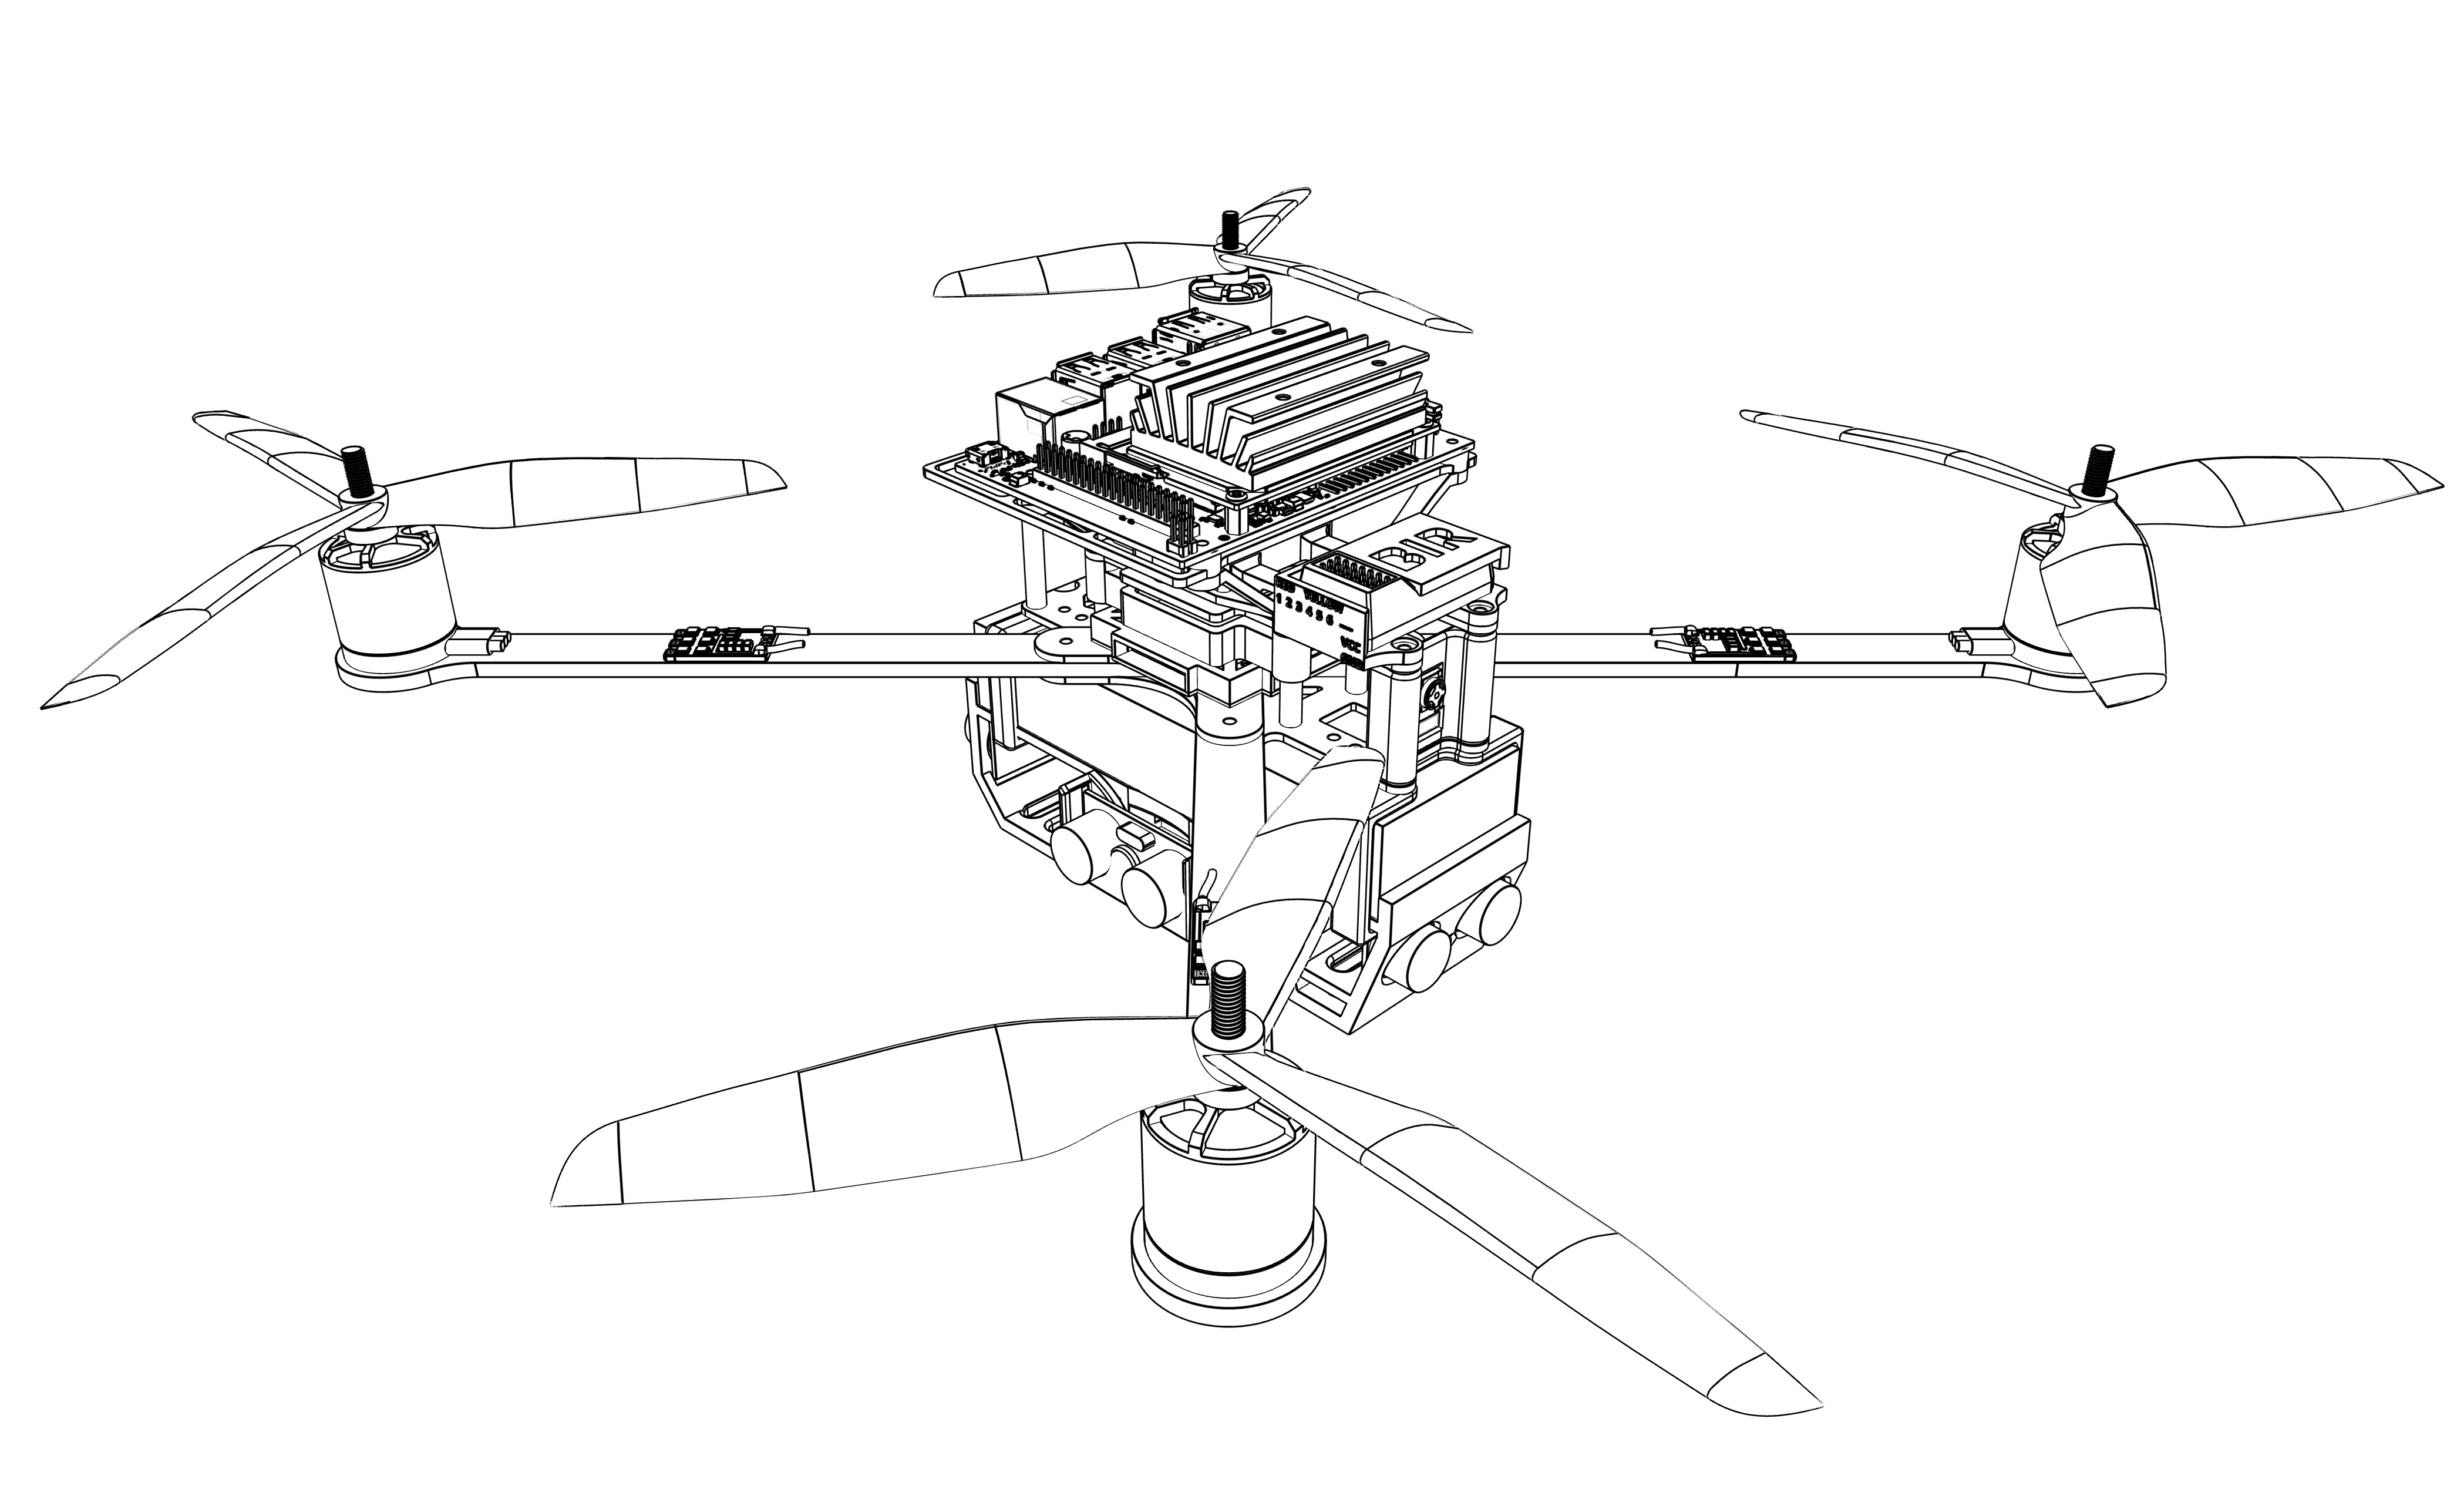
\includegraphics[width=1\textwidth]{img/carcara2.png}
%                 \label{fig:carcara2}
%             \end{figure}
%         \end{column}
%     \end{columns}
% \end{frame}

